\documentclass[12pt,fleqn]{article}\usepackage{../../common}
\begin{document}
Materyel Mekaniği - 2

Kirişin Yatay Kesme Stresi

Yatay kesme stresinin mevcut olduğunun belki de en iyi ispatı alttaki şekli
göstermek. İki tane tıpatıp aynı kirişi üst üste koysak ve üstten bir $P$ yükü
uygulasak, eğer kirişler arası sürtünme çok az ise kirişler birbirinden ayrı
şekilde büküleceklerdi, (b) şeklinde görüldüğü gibi.

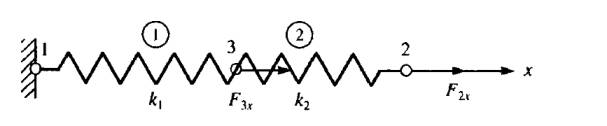
\includegraphics[width=15em]{phy_020_strs_02_02.jpg}

Şimdi hayal edelim ki kirişler birbirine tutkal ile yapıştırıldı, bu şekilde iki
parça tek bir parça haline geldi. Bu birleşik kiriş yüklendiğinde o yapıştırılan
yatay yüzeyde stresler oluşmalıdır ki yapıştırılmış yüzeyin üst (b) şekildeki
gibi kayması engellensin. Bu kesme stresleri sayesinde tek birleşik kiriş ayrı
ayrı iki kirişten daha katıdır / serttir (stiff). Aynı kavram genel olarak
moleküler yapışma ile tek parça nesnelere de uygulayanabilirdi. Bir vidaya dikey
yönde uygulanan yük kesme yönünde stres yaratır, ki bu stresler moleküler
bağlantılar üzerinden ortaya çıkar.

Türetmeye gelelim [2, sf. 388]. Birörnek bükülmeye maruz olan bir kirişi
düşünelim, yine üstteki (a) resmini referans alıyoruz, bu kirişte $\ud x$
genişliğindeki ufak bir parçaya odaklanalım, bu ufak parçanın sol kısmına etki
eden kesme kuvveti ve bükülme momenti $V$ ve $M$. Eksende sağa gittikçe bu
değerler değişik olabileceği için parçanın sağında $V + \ud V$ ve $M + \ud M$
olacaktır.

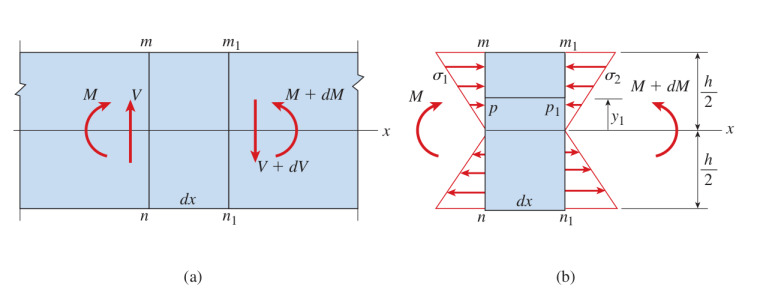
\includegraphics[width=30em]{phy_020_strs_02_01.jpg}

$\sigma_1$ ve $\sigma_2$ formüllerini yazalim, bükülme normal stres (flexure)
formülünden $\sigma = My / I$ olduğunu biliyoruz,

$$
\sigma_1 = -\frac{My}{I}, \quad
\sigma_2 = \frac{(M + \ud M)y}{I}
$$

Üstteki (b) resminde daha da ufak bir bölgeye odaklanalım, alttaki (c)
resminde daha net gösteriliyor,

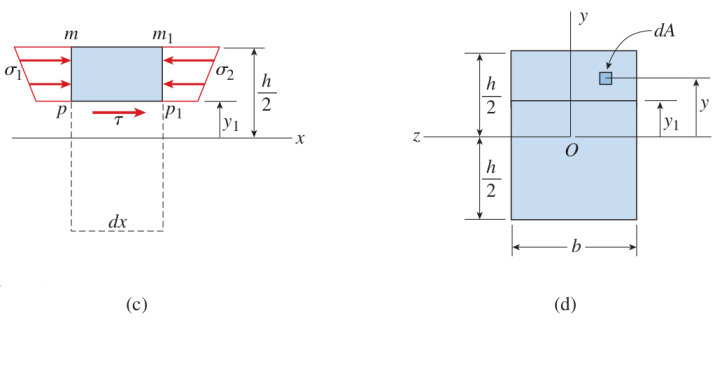
\includegraphics[width=30em]{phy_020_strs_02_03.jpg}

Bu parçanın en üst kısmı kirişin en üstü, orada yatay kesme stresi yok.
Parçanın alt kısmındaki strese $\tau$ diyelim. (c) figürünün sol taraftan
bakılan hali (d) resminde. Kuvvetleri düşünürsek, $F_1,F_2,F_3$ diyelim alttaki
gibi olur.

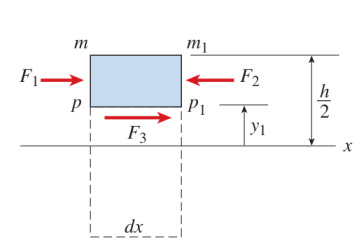
\includegraphics[width=15em]{phy_020_strs_02_04.jpg}

Denge açısından

$$
F_3 = F_2 - F_1
$$

olmalıdır.

Bu kuvvetleri yerine koyalım o zaman, mesela $\sigma_1$'den hareketle,

$$
\sigma_1 \ud A = \frac{My}{I} \ud A
$$

Tüm $F_1$ kuvveti için tanımladığımız alan üzerinden entegral alalım,

$$
F_1 = \int \sigma_1 \ud A = \int \frac{My}{I} \ud A
$$

$F_2,F_3$ için benzer şekilde,

$$
F_2 = \int \sigma_2 \ud A = \int \frac{(M + \ud M)y}{I} \ud A
$$

$$
F_3 = \int \frac{(M + \ud M)y}{I} \ud A -  \int \frac{My}{I} \ud A =
\int \frac{(\ud M)y}{I} \ud A
$$

$$
F_3 = \frac{\ud M}{I} \int y \ud A
$$

$F_3$'e farklı bir açıdan yaklaşalım, eğer $b$ boyunca kesme stresi $\tau$
değişmiyor ise, o zaman $F_3$'ü alttaki gibi de belirtebilirdik,

$$
F_3 = \tau b \ud x
$$

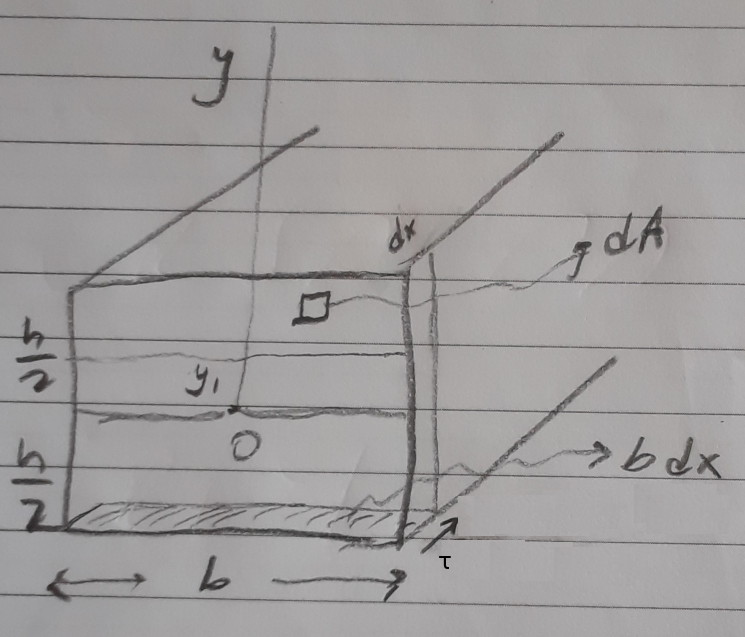
\includegraphics[width=15em]{phy_020_strs_02_05.jpg}

Kuvvet eşittir stres çarpı alandır, $b \ud x$ ile belirtilen alan üstteki
resimde görülüyor, kirişin altındaki eni $b$ boyu $\ud x$ olan bölgeden
bahsediyoruz. Burada $\tau$ sabit ise üstteki çarpım yapılabilir, tabii ki
$\tau$ büyüklüğü $y$'ye bağlı olduğu için aşağı, yukarı değişimde $\tau$
değişirdi.

Devam edelim, son iki formülü birleştirince

$$
\frac{\ud M}{I} \int y \ud A = \tau b \ud x
$$

Tekrar düzenleyince

$$
\tau = \frac{\ud M}{\ud x} \left( \frac{1}{Ib}  \right) \int y \ud A
$$

$\ud M / \ud x$ büyüklüğü kesme kuvveti $V$'ye eşittir. 

$$
\tau =  \frac{V}{Ib} \int y \ud A
$$

$\int y \ud A$ entegrali $Q$ ile gösterilir, alansal bir momenttir, yine kiriş
yan yüzey şekli ile alakalı, standart şekiller için bilinen formüller vardır, o
zaman nihai formül

$$
\tau =  \frac{VQ}{Ib}
$$

Kirişin Yatay Kesme Stresi - Alternatif Anlatım

Kesme stresi $\tau$'yu bulmak için yine kirişin ufak bir kısmına odaklanalım,

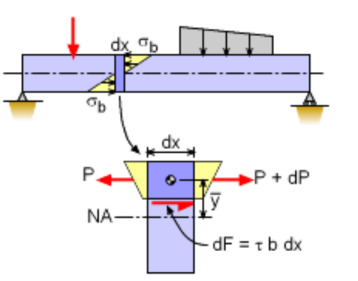
\includegraphics[width=15em]{phy_020_strs_02_09.jpg}

Tüm etki eden kuvvetlerin toplamı sıfır olmak zorundadır [3],

$$
-P + (P + \ud P) + \tau b \ud x = 0
$$

ki $b$ kesme stresinin uygulandığı noktadaki kiriş derinliğidir. 

$$
-\ud P/\ud x = \tau b
\mlabel{1}
$$

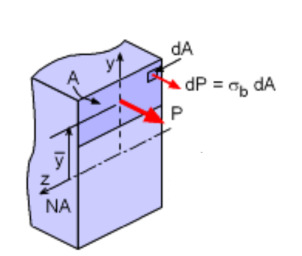
\includegraphics[width=15em]{phy_020_strs_02_10.jpg}

$P$'yi bulmak için $A$ bölgesindeki stresleri entegre ediyoruz,

$$
\int_A \ud P = \int_A \sigma_b \ud A
$$

Fakat daha önce bulduk ki $\sigma_b = -My / I$, yerine koyunca,

$$
P = \int_A - \frac{My}{I} \ud A
$$

$M$ ve $I$ sabittir, entegral dışına çıkartılabilir,

$$
P = - \frac{M}{I} \int_A y \ud A = - \frac{MQ}{I}
$$

ki görülen entegral bir alanın kütle merkezini bulmak için kullanılan standart
bir entegraldir, $Q = \int_A y \ud A$. Devam edelim üstte bulunan $P$'yi (1)'e
sokunca,

$$
- \frac{\ud}{\ud x} \left( - \frac{MQ}{I} \right) = \tau b
$$

$$
\frac{Q}{I} \frac{\ud M}{\ud x} = \tau b
$$

Şimdi hatırlarsak $\ud M/\ud x$ türevi yatay kesme / teğetsel yükü $V$'ye
eşittir. O zaman

$$
\frac{Q}{I} V = \tau b
$$

Nihai yatay kesme stres denklemi,

$$
\tau = \frac{V Q}{I b}
$$

Problemler

Altta kiriş odaklı bazı örnek problemleri çözeceğiz. Bir kirişe yük
uygulandığında dengenin muhafaza edilmesi için kiriş içinde kuvvetler oluşur.
Bu iç kuvvetler kirişin destek yapısına göre farklı şekillerde ortaya çıkabilir
[1].

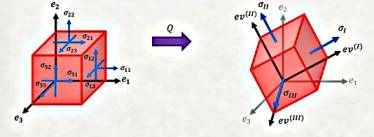
\includegraphics[width=25em]{phy_020_strs_02_08.jpg}

Üstteki soldaki resimde mesela iki boyutta pimli destek dönüşe izin verir,
tekerlekli yatay sağ, sol hareketi ve dönüşü serbest bırakır. Sabit destekte hiç
harekete izin yoktur. Hangi harekete izin verilmediğine göre yük uygulanması
ardından üst sağdaki iç kuvvetler ortaya çıkacaktır, bunlar pimli durumda dikey
ve yatay kuvvetler, tekerlekli durumda dikey kuvvet, sabit durumda ise her üç
mümkün tepkilerdir, yani moment, dikey ve yatay.

Yükler noktasal ya da dağıtık şekilde uygulanabilir, altta noktasal kuvvet,
dağıtık kuvvet ve noktasal moment örneklerini görüyoruz.

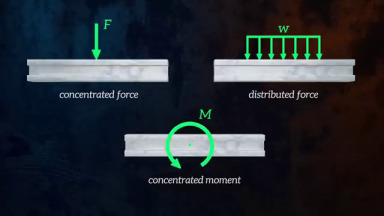
\includegraphics[width=20em]{phy_020_strs_02_07.jpg}

Tipik olarak problemin beklediği kesim kuvveti ve bükülme momenti grafikleridir,
bu grafiklerde $x$ ekseni yatay olarak kirişin kendisi, $y$ ekseni ise o noktada
etki eden kesim ya da moment büyüklüğüdür.

Çözme yöntemi olarak iki yaklaşım mevcut, biri her kritik noktada kirişin
hissettiği içsel kuvvetler ve momentleri hesaplamak için o noktalarda denge
denklemlerini kullanmak, ki bu denklemlere (ve temel fiziğe göre) kirişe
uyguladığımız hayali bir kesitte etki eden tüm kuvvetler ve momentler birbirini
dengelemeli. Ardından bu kesit tüm kiriş boyunca kaydırılır ve gereken kuvvetler
aynı denge üzerinden hesaplanır. Eğer tüm yükler noktasal ise bu yaklaşım iyi
işler.

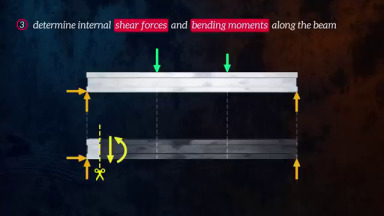
\includegraphics[width=20em]{phy_020_strs_02_06.jpg}

Bir diğer yaklaşım Calculus kullanmak. Bu yaklaşım temelde sürekli bazda çözüm
verdiği için dağıtık yük durumunda daha kolay işler, kritik noktalara odaklanmak
yerine pür formulsel düşünebiliriz . Daha önce görmüştük ki kesim kuvvet
formülünün eğimi (türevi) o noktadaki uygulanan yükün negatifidir $\ud V / \ud x
= -w$, ve bükülme moment grafiğinin eğimi ise o noktadaki kesim kuvvetine
eşittir, $\ud M / \ud x = V$. Şimdi ters yönde gidersek, ilk formülü entegre
edince mesela iki nokta arasındaki kesme kuvveti farkının yükleme eğrisinin
altında kalan aynı noktalar arasındaki alanın olduğunu görebilirdik.

$$
V_2 - V_1 = - \int_{x_1}^{x_2} w \ud x
$$

İkinci formülü entegre edince iki nokta arasındaki bükülme moment farkının kesme
kuvveti eğrisinin altında kalan alanın olduğunu bulurduk [1].

$$
M_2 - M_1 = \int_{x_1}^{x_2} V \ud xa
$$







Problem 1

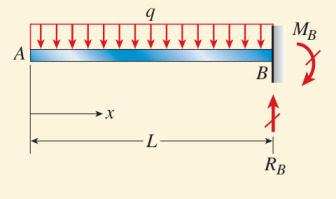
\includegraphics[width=20em]{phy_020_strs_02_11.jpg}

Üstüne birörnek yük $q$ uygulanan bir dirsekli (cantilever) kiriş için kesme
kuvveti ve bükülme momenti diyagramı çizin [2, sf. 334].

Çözüm

$$
V - V_A = V - 0 = V = -\int_{0}^{x} q \ud x = -qx
$$

$$
M - M_A = M - 0 = M = \int_{0}^{x} -qx \ud x = -\frac{qx^2}{2}
$$

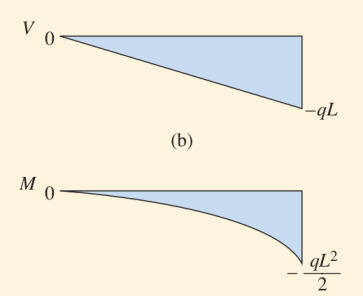
\includegraphics[width=20em]{phy_020_strs_02_12.jpg}

Kaynaklar 

[1] The Efficient Engineer, {\em Understanding Shear Force and Bending Moment Diagrams},
    \url{https://youtu.be/C-FEVzI8oe8}

[2] Gere, {\em Mechanics of Materials, 7th Edition}

[3] Gramoll, {\em Mechanics},
    \url{http://www.ecourses.ou.edu/cgi-bin/ebook.cgi?topic=me}

\end{document}

